\section{Evaluation Framework}
\label{sec:eval_frameworks}
% \KZ{Are we only evaluating the final version of the two bots from prev section? This is not part of the iterative design process right? This should be made clearer.}
% \MY{normally we provide objective/automatic eva first, followed by human evaluation results. when introducing the metrics and results, follow this order}

This section describes our evaluation framework, covering interactive experiments for ``human-bot'' chats, along with diverse task-specific metrics. Aligned with proposed objectives, this framework can be applied to evaluate the performance of various psychiatrist and patient chatbots.

\subsection{``Human-bot'' Interactive Chat}
The human evaluation measure is widely considered as golden metric for dialog system. In contrast to the approach of using actors/actresses to simulate patients as mentioned in \citet{yao-etal-2022-d4}, our evaluation process involves \textit{actual depression patients} interacting with psychiatrist chatbot and \textit{human psychiatrists} interacting with patient chatbot. 
This approach allows us to evaluate the performance of these two types of chatbots in real-world scenarios.
We introduce our participants as follows:

\paragraph{Depressive individuals} were recruited through online advertisements, resulting in the participation of 14 volunteers aged 18 to 31. The gender distribution was 28.57\% male and 71.43\% female. 

\paragraph{Psychiatrists} were invited through cooperation with hospitals. We invited 9 psychiatrists, two of them are graduate students majoring in psychiatry, and the rest are practicing psychiatrists with rich clinical experience to ensure the professionalism of the evaluation.

\paragraph{Evaluation Procedure}
We adhere to standard human evaluation procedures~\cite{Yue2023Beyond}, where each participant engages with all the chatbots in random order, and rates their performance after a full conversation with each one. Once participants conclude interactions with all chatbots, they are instructed to adjust their original ratings to ensure that each chatbot receives different scores in the same metric. 

\subsection{Evaluation Metrics}
\label{sec:eval_metric}
When designing evaluation metrics, our goal is to ensure that each objective is accompanied by appropriate metrics for accurate measurement.  We employ both rating and computational metrics for evaluation. \textbf{Rating metrics} are scored by humans after interactive conversations with the chatbot, while \textbf{computational metrics} can be calculated based on the dialog history.  
We divide the computational metrics of both kind of chatbots into two types: \textit{function} and \textit{style}. The overview of these metrics and their relations to objectives can be found in \figref{fig:all_metric}.
% \MY{Clearer now, but still mixing function and style - which objectives and metrics are function-related and which are style?}.
% NEWCOMMENT: 这里这样分类之后,在图中也要把两类指标区分出来,可以在objective那一列上做区分
\begin{figure}[th]
	\centering
	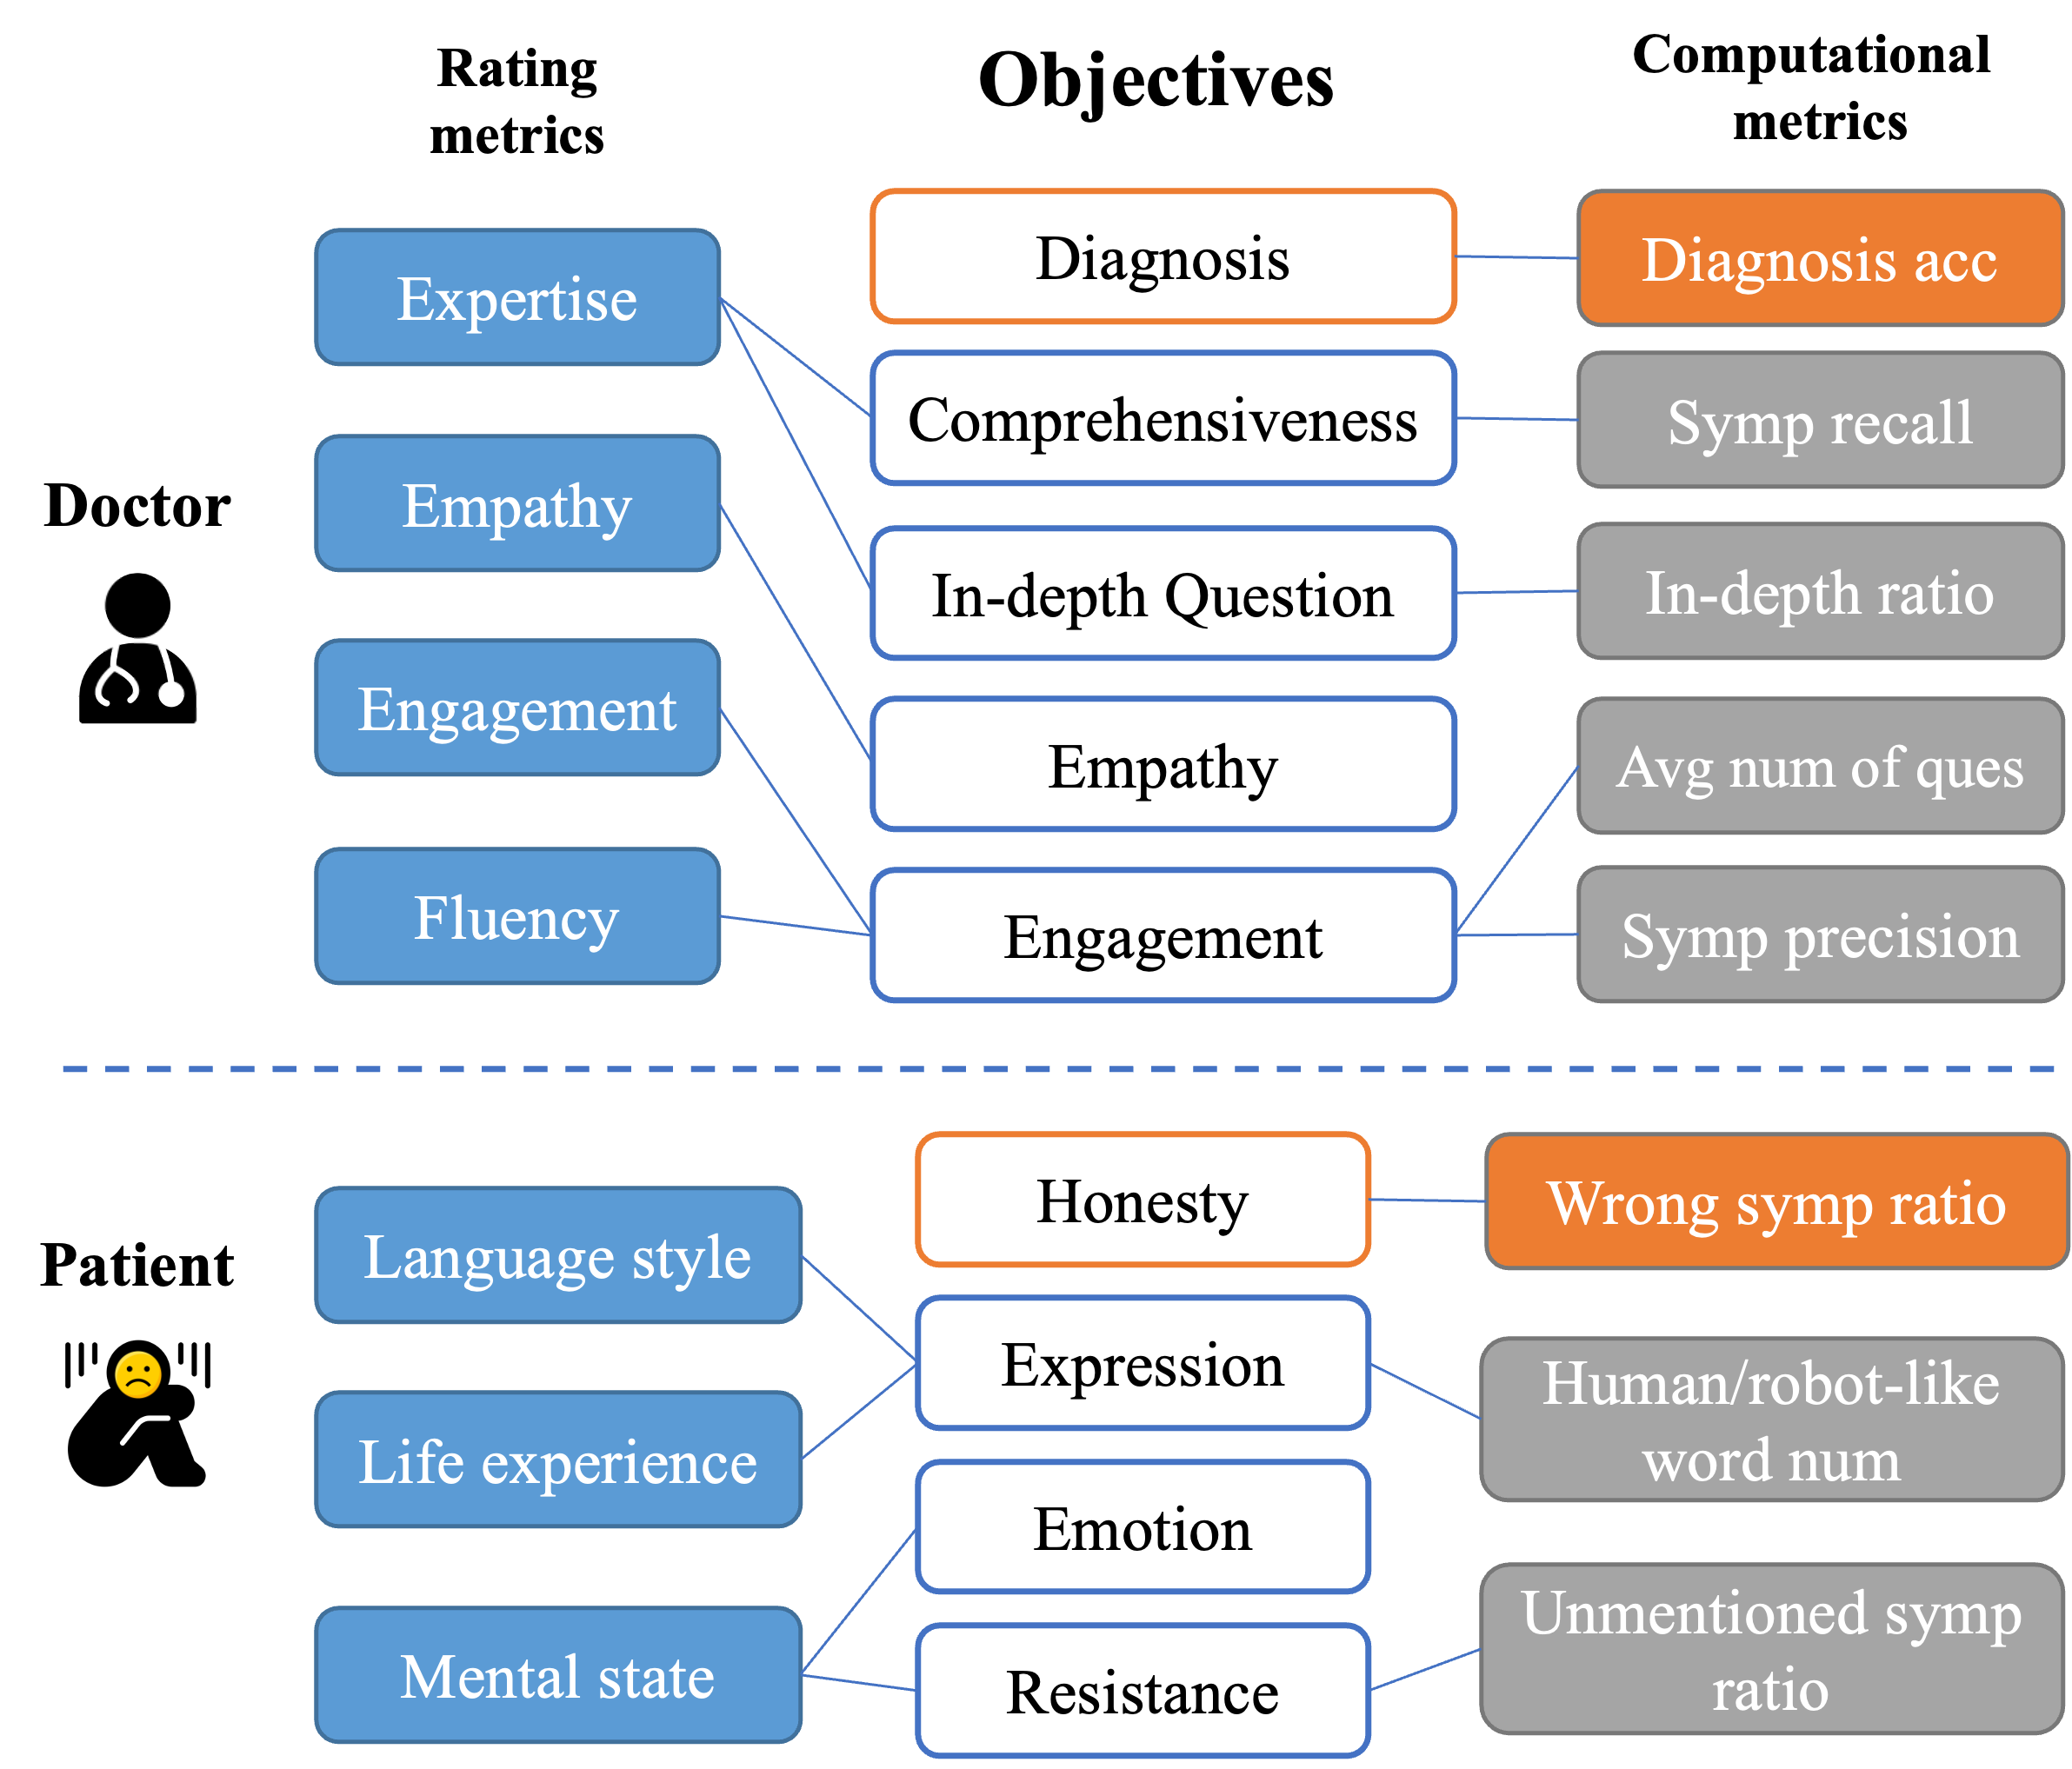
\includegraphics[width=\linewidth]{Figures/metrics_new.png}
	\caption{The correspondence between evaluation metrics and objectives. \textbf{\textit{Function}} metrics are orange, and \textbf{\textit{style}} metrics are gray.}
	\label{fig:all_metric}
\end{figure}

\subsubsection{Metrics for Psychiatrist Chatbot}
\paragraph{Rating Metrics} 
We mainly focus on the user experience for rating metrics of psychiatrist chatbot, as shown in Table \ref{tab:human_eval_doctor}. This emphasis stems from the fact that, in most cases, patients lack specialized knowledge in psychiatry, making it challenging for them to precisely assess a doctor's professional skills.
% In most cases, patients do not have specialized knowledge in psychiatry, making it difficult for them to assess a doctor's professional skills precisely. Therefore, we focus mainly on the user experience for rating metrics of psychiatrist chatbot, as shown in Table \ref{tab:human_eval_doctor}.
\begin{table}[h]
    \centering
    \footnotesize
    \begin{tabular}{m{0.18\columnwidth}|m{0.7\columnwidth}}
    \hline
    Metrics & Explanation \\
    \hline
    Fluency & The chatbot does not repeat previously asked questions and can smoothly switch between different topics. \\
    \hline
    Empathy & The chatbot can understand and comfort you properly. \\
    \hline
    Expertise & The chatbot behaves like a real doctor, making you believe in its professionalism. \\
    \hline
    Engagement & The chatbot can maintain your attention and make you want to continue talking to it. \\
    \hline
    \end{tabular}
    \caption{Rating metrics of psychiatrist chatbot.}
    \label{tab:human_eval_doctor}
\end{table}
\paragraph{Computational Metrics}
Different from rating metrics, we mainly measure the expertise of the psychiatrist chatbot using computational metrics based on dialog history.
The \textit{functional} requirements for psychiatrist chatbot is to provide an accurate diagnosis, so the corresponding metric is \uline{``diagnosis accuracy''}. 
The \textit{style} part concerns the psychiatrist chatbot's professional skills. We use \uline{``symptom recall''} to evaluate the chatbot's ability to comprehensively gather the patient's symptom-related information, and use \uline{``in-depth ratio''} to assess the ability to ask in-depth questions for deeper understanding. 
To ensure a better user experience, we calculate the \uline{``average number of questions''} asked in a single interaction to discourage the chatbot from overwhelming patients with excessive queries. Furthermore, we employ the metric of \uline{``symptom precision''} to penalize the chatbot's mechanistic behavior of asking all potential questions, irrespective of the user's responses\footnote{A detailed explanation of these computational metrics can be found in Appendix \ref{apd:eval}.\label{footnote:comp_metric}}. 

\subsubsection{Metrics for Patient Chatbot}
\paragraph{Rating Metrics}
There is no standard to measure whether a patient is ``good'' enough. Thus, when chatting with patient chatbots, doctors can only assess whether their style of expression and manner of communication resemble real patients enough and whether they can describe their symptoms in a reasonable way, so the main metrics for rating are \textbf{Resemblance} and \textbf{Rationality}.
We further divide the Resemblance metric into three aspects in Table \ref{tab:human_eval_patient}, according to the objectives in Section \ref{sec:objectives}.

\begin{table}[h]
    \centering
    \footnotesize
    \begin{tabular}{m{0.18\columnwidth}|m{0.65\columnwidth}}
    \hline
    Metrics & Explanation \\
    \hline
    Mental State & The chatbot is in depressed state, such as be in low mood, reluctance to communicate, scattered thoughts, etc.\\
    \hline
    Life Experience & The description of symptoms is related to daily life and personal experiences.\\
    \hline
    Language Style & Use colloquial and natural expressions when describing symptoms.\\
    \hline
    \end{tabular}
    \caption{Three aspects of the ``Resemblance'' metric.}
    \label{tab:human_eval_patient}
\end{table}
\paragraph{Computational Metrics}
The \textit{functional} requirement of patient chatbot is ``honesty'', and we can calculate \uline{``wrong symptom ratio''} by comparing the patient's symptom list with the symptoms it reported to assess this aspect. 

Then, we evaluate the patient chatbots' \textit{style} using some linguistic features, like \uline{``Human/robot-like word ratio''}, to find out whether their language is colloquial with limited usage of professional terminology. We also use \uline{``unmentioned symptom ratio''} to measure the resistance level of chatbots\textsuperscript{\ref{footnote:comp_metric}}. 

% \subsection{Human Evaluation}
% The human evaluation measure is widely considered as golden metric for dialog system. In contrast to the approach of using actors/actresses to simulate patients as mentioned in \citet{yao-etal-2022-d4}, our human evaluation process involves actual depression patients, enabling us to assess the performance of chatbots in real-world scenarios.

% Depression patients were recruited through online advertisements, resulting in the participation of 14 volunteers aged 18 to 31. The gender distribution was 28.57\% male and 71.43\% female. 

% First, to assess the severity of participants' depression, they were asked to complete the Beck Depression Inventory~\cite{beck1996beck}, yielding a score ranging from 0 to 63. Notably, we have a balanced distribution of subjects across various depression levels: $healthy_{(0-13)}$, $mild_{(14-19)}$, $moderate_{(20-28)}$ and $severe_{(29-63)}$ according to the Beck Depression Score\footnote{Refer to Table \ref{tab:distribution_seve} in Appendix \ref{apd:eval} for the distribution details.}.
% We adhere to standard human evaluation procedures~\cite{Yue2023Beyond}, where each participant engages with all the psychiatrist chatbots in random order, and rates their performance after a full conversation with each one. Once participants conclude interactions with all chatbots, they are instructed to adjust their original ratings to ensure that each chatbot receives different scores in the same metric. 

% We carefully design human evaluation metrics \KZ{sentence incomplete.}

\subsection{Computation and Annotation}
% A detailed explanation of the automatic metrics for the doctor and patient chatbot can be found in Appendix \ref{apd:eval}. \MY{This sentence can put in footnote, a bit distracted to start a new subsection with reference to appendix. Say things like "We establish comprehensive and quantitative metrics like xx, xx, and xxx, each covering xx xx aspects. footnote, details can be found in ..."}

To obtain the ground truth score of the metrics ``diagnosis accuracy'', each participant engaging with our psychiatrist chatbot is invited to complete the Beck Depression Inventory~\cite{beck1996beck} to evaluate the severity of their depression.

In addition, to calculate some of these metrics, we need to annotate the dialog history. This involves identifying the relevant symptom in the doctor's question, determining whether the patient truly experiencing a certain symptom, and so on, which is described in Appendix \ref{apd:annotation}.

% First, to assess the severity of participants' depression, they were asked to complete the Beck Depression Inventory~\cite{beck1996beck}, yielding a score ranging from 0 to 63. Notably, we have a balanced distribution of subjects across various depression levels: $healthy_{(0-13)}$, $mild_{(14-19)}$, $moderate_{(20-28)}$ and $severe_{(29-63)}$ according to the Beck Depression Score\footnote{Refer to Table \ref{tab:distribution_seve} in Appendix \ref{apd:eval} for the distribution details.}.

% Due to the inadequacy of dialogue history data for training multiple classification models, we employ ChatGPT to automatically label each sentence in the dialogue history, leveraging its impressive annotation capabilities~\cite{Gilardi2023ChatGPTOC}. Subsequently, three annotators thoroughly review and rectify the results to ensure the quality of the annotation.
% To assess the performance of dialogue systems, it is crucial to employ both human evaluation and automatic metrics, especially in mental health domain. Since there is little previous work on how to evaluate simulated psychiatrists and patients, we design several task-specific metrics and interactive experiments for human evaluation. 

% \subsection{Human Evaluation Participants}
% % We first implemented a website to host our chatbots, making it easier for participants to interact with them and rate their performance. The details of the website can be found in Appendix \ref{sec:chatInterface}. 
% %\subsubsection{Participants}
% In contrast to the approach of using actors/actresses to simulate patients as mentioned in \citet{yao-etal-2022-d4}, our evaluation process involves actual depression patients and psychiatrists, enabling us to assess the performance of chatbots in real-world scenarios.

% Depression patients are recruited through online advertisements.
% A total of 14 volunteers completed the entire process. Their age ranges from 18 to 31, while 4 of them are male, while the rest of female. 
% To assess the severity of their depression, patients are asked to complete the Beck Depression Inventory~\cite{beck1996beck}. Notably, we have a balanced distribution of healthy, mild, moderate and severe depression subjects which distribution is presented in Table \ref{tab:distribution_seve} in Appendix \ref{apd:eval}.
% % \KZ{If the severity is ``none'', this patient is considered healthy?}

% We invited 9 psychiatrists who are not involved in the prompt design, through cooperation with hospitals. Two of them are graduate students majoring in psychiatry, and the rest are practicing psychiatrists with rich clinical experience to ensure the professionalism of the evaluation.